\section*{Chapter 7}

\subsection*{Exercise 7.1}
In Chapter 6 we noted that the Monte Carlo error can be written as the
sum of TD errors (6.6) if the value estimates don't change from step to step. Show that
the n-step error used in (7.2) can also be written as a sum of TD errors (again if the
value estimates don't change) generalizing the earlier result. 

\subsubsection*{Solution:}

\begin{align*}
    G_{t:t+n} - V(S_t) &= R_{t+1} + \gamma G_{t+1:t+n} - V(S_t) + \gamma V(S_{t+1}) - \gamma V(S_{t+1}) \\
    &= \delta_t + \gamma (G_{t+1:t+n} - V(S_{t+1})) \\
    &= \delta_t + \gamma \delta_{t+1} + \gamma^2 (G_{t+2:t+n} - V(S_{t+2})) \\
    &= \delta_t + \gamma \delta_{t+1} + \gamma^2 \delta_{t+2} + \cdots + \gamma^{n-1} \delta_{t+n-1} \\
    &= \sum_{k=t}^{t+n-1} \gamma^{k-t} \delta_k
\end{align*}


\subsection*{Exercise 7.2 (programming)}
With an n-step method, the value estimates do change from
step to step, so an algorithm that used the sum of TD errors (see previous exercise) in
place of the error in (7.2) would actually be a slightly different algorithm. Would it be a
better algorithm or a worse one? Devise and program a small experiment to answer this
question empirically.

\subsubsection*{Solution:}

See the notebook.
The experiment involves the random walk problem mentioned in the book. The implementation of the algorithm using the sum of TD errors might not be right, as the point where the state values need to be updated and the calculation of $\delta$'s are not clear to me.
Looking aside from that, the algorithm using the sum of TDs should be worse, as they have a higher variance and (in this case) diverge for larger $\alpha$ values.
\begin{figure}[H]
    \centering
    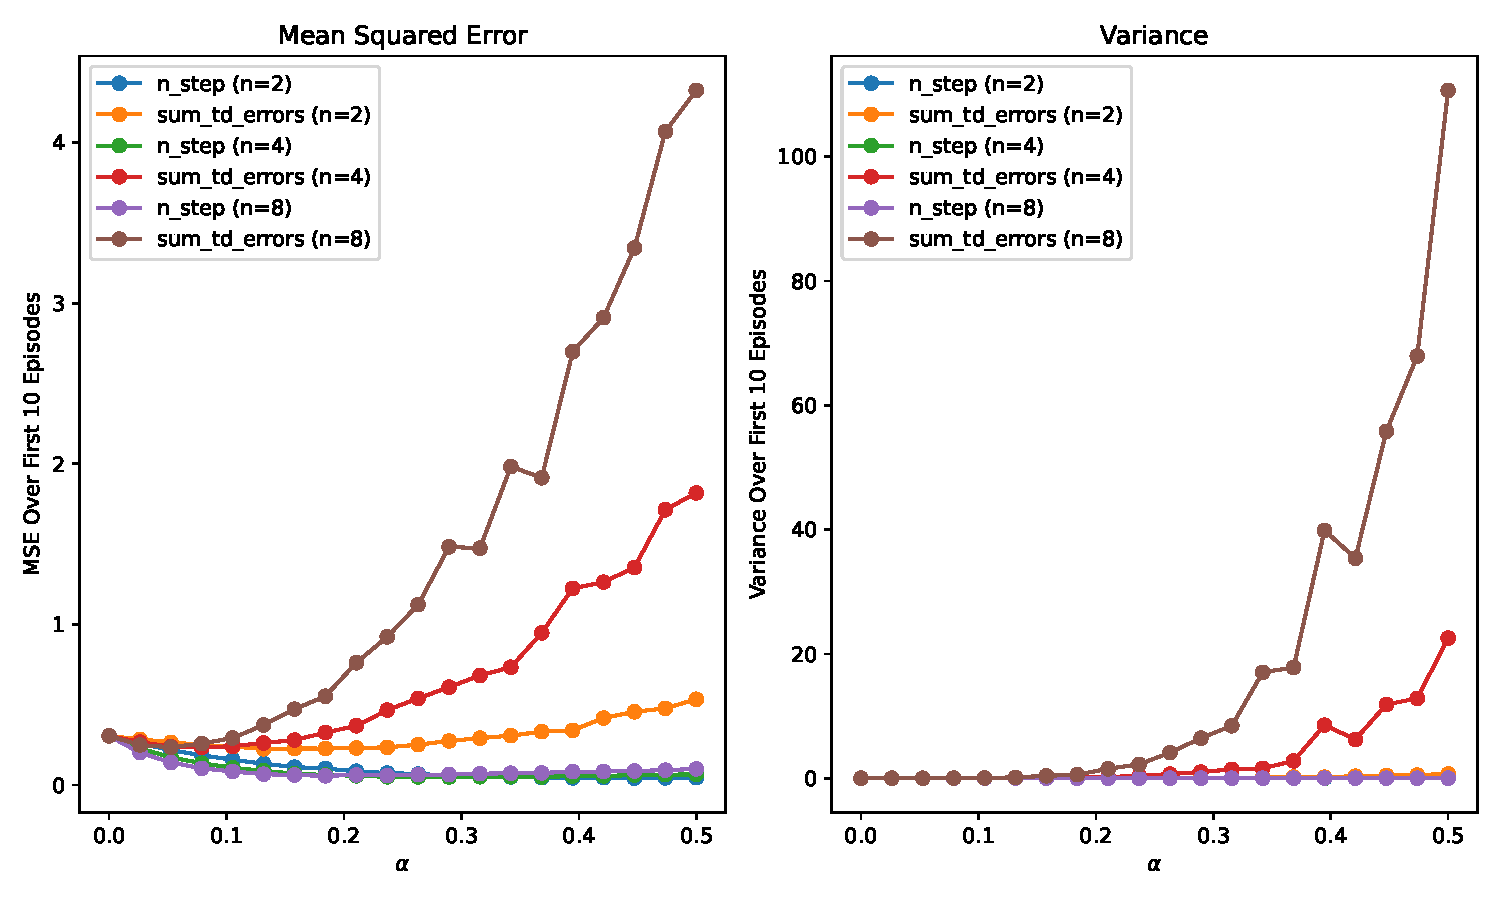
\includegraphics[width=0.8\textwidth]{chapters_latex/figures/ex_07_02.pdf}
    \captionsetup{labelformat=empty}
    \caption{Mean and variance of the MSE after 10 episodes, averaged over 100 runs.}
\end{figure}

\subsection*{Exercise 7.3}
Why do you think a larger random walk task (19 states instead of 5) was
used in the examples of this chapter? Would a smaller walk have shifted the advantage
to a different value of n ? How about the change in left-side outcome from 0 to -1 made
in the larger walk? Do you think that made any difference in the best value of n?

\subsubsection*{Solution:}
The larger task is used to better illustrate the effects of different $n$-step methods due to longer episodes.

With a smaller walk, the advantage would have shifted to a different value of $n$, as the optimal $n$ depends on the length of the episodes.

The change in the left-side outcome from 0 to $-1$ made in the larger walk does not make any difference in the best value of $n$, as the updates are the same, just linearly shifted.

\subsection*{Exercise 7.4}
Prove that the n-step return of Sarsa (7.4) can be written exactly in terms
of a novel TD error, as
\[
G_{t:t+n} = Q_{t-1}(S_t, A_t) + \sum_{k=t}^{\min(t+n, T) - 1} \gamma^{k-t} \left[ R_{k+1} + \gamma Q_k(S_{k+1}, A_{k+1}) - Q_{k-1}(S_k, A_k) \right].
\]

\subsubsection*{Solution:}

\begin{align*}
    G_{t:t+n} &= R_{t+1} \\
    &+ \gamma R_{t+2} \\
    &+ \gamma^2 R_{t+3} \\
    &\cdots \\
    &+ \gamma^{n-1} R_{t+n} \\
    &+ \gamma^n Q_{t+n-1}(S_{t+n}, A_{t+n})  \\
    &= R_{t+1} + Q_{t-1}(S_{t}, A_{t}) - Q_{t-1}(S_{t}, A_{t}) \\
    &+ \gamma R_{t+2} + \gamma  Q_{t}(S_{t+1}, A_{t+1}) -\gamma  Q_{t}(S_{t+1}, A_{t+1})\\
    &+ \gamma^2 R_{t+3} + \gamma^2 Q_{t+1}(S_{t+2}, A_{t+2}) -\gamma^2  Q_{t+1}(S_{t+2}, A_{t+2}) \\
    &\cdots \\
    &+ \gamma^{n-1} R_{t+n} + \gamma^{n-1}Q_{t+n-2}(S_{t+n-1}, A_{t+n-1}) - \gamma^{n-1}Q_{t+n-2}(S_{t+n-1}, A_{t+n-1}) \\
    &+ \gamma^n Q_{t+n-1}(S_{t+n}, A_{t+n}) \\
    &= Q_{t-1}(S_t, A_t) \\
    &+ R_{t+1} + \gamma Q_t(S_{t+1}, A_{t+1}) - Q_{t-1}(S_t, A_t) \\
    &+ \gamma R_{t+2} + \gamma^2 Q_{t+1}(S_{t+2}, A_{t+2}) - \gamma Q_t(S_{t+1}, A_{t+1}) \\
    &+ \gamma^2 R_{t+3} + \gamma^3 Q_{t+2}(S_{t+3}, A_{t+3}) - \gamma^2 Q_{t+1}(S_{t+2}, A_{t+2}) \\
    &\cdots \\
    &+ \gamma^{n-1} R_{t+n} + \gamma^n Q_{t+n-1}(S_{t+n}, A_{t+n}) - \gamma^{n-1} Q_{t+n-2}(S_{t+n-1}, A_{t+n-1}) \\
    &= Q_{t-1}(S_t, A_t) + \sum_{k=t}^{\min(t+n, T) - 1} \gamma^{k-t} \left[ R_{k+1} + \gamma Q_k(S_{k+1}, A_{k+1}) - Q_{k-1}(S_k, A_k) \right].
\end{align*}


\subsection*{Exercise 7.5}
Write the pseudocode for the off-policy state-value prediction algorithm
described above.

\subsubsection*{Solution:}

\fbox{
\begin{minipage}{0.95\textwidth}
\footnotesize
Input: policies $\pi$ and \textcolor{blue}{$b$ (a behavior policy)}

Algorithm parameters: step size $\alpha \in (0,1]$, a positive integer $n$

Initialize $V(s)$ arbitrarily, for all $s \in \mathcal{S}$

All store and access operations (for $S_t$ and $R_t$) can take their index mod $n+1$\\


\textcolor{blue}{
Define function $\bar{G}(t, h)$ as:
\begin{itemize}[left=0em]
    \item[] if $t = h$: return $V(S_h)$
    \item[] if $t = T$: return $0$
    \item[] else: return $\rho_t(R_{t+1} + \gamma \bar{G}(t+1, h)) + (1-\rho_t) V(S_t)$
\end{itemize}
}

Loop for each episode:
\begin{itemize}[left=0em]
    \item[] Initialize and store $S_0 \neq$ terminal
    \item[] $T \leftarrow \infty$
    \item[] Loop for $t = 0, 1, 2, \dots$:
    \begin{itemize}[left=0em]
        \item[] If $t < T$, then:
        \begin{itemize}[left=0em]
            \item[] Take an action according to $b(\cdot | S_t)$
            \item[] \textcolor{blue}{$\rho_t \leftarrow \pi(A_t | S_t) / b(A_t | S_t)$}
            \item[] Observe and store the next reward as $R_{t+1}$ and the next state as $S_{t+1}$
            \item[] If $S_{t+1}$ is terminal, then $T \leftarrow t+1$
        \end{itemize}
        \item[] $\tau \leftarrow t - n + 1$ \hspace{1cm} ($\tau$ is the time whose state's estimate is being updated)
        \item[] If $\tau \geq 0$:
        \begin{itemize}[left=0em]
            \item[] \textcolor{blue}{$G \leftarrow \bar{G}(\tau, \tau+n)$}
            \item[] $V(S_{\tau}) \leftarrow V(S_{\tau}) + \alpha \left[ G - V(S_{\tau}) \right]$
        \end{itemize}
    \end{itemize}
\end{itemize}
Until $\tau = T - 1$

\end{minipage}
}


\subsection*{Exercise 7.6}
Prove that the control variate in the above equations does not change the
expected value of the return.

\subsubsection*{Solution:}
\[
    \mathbb{E}_b \left[ (1 - \rho_t) V_{h-1}(S_t) \right]  = \mathbb{E}_b \left[ (1 - \rho_t) \right] \mathbb{E}_b \left[ V_{h-1}(S_t) \right]  = 0
\]
and

\begin{align*}
    &\mathbb{E}_b \left[ \bar{V}_{h-1}(S_{t+1}) - \rho_{t+1} Q_{h-1}(S_{t+1}, A_{t+1}) \big| S_{t+1} \right] \\
    &= \sum_a \pi(a | S_{t+1}) Q_{h-1}(S_{t+1}, a) - \sum_a b(a | S_{t+1}) \frac{\pi(a | S_{t+1})}{b(a | S_{t+1})} Q_{h-1}(S_{t+1}, a) \\
    &= 0
\end{align*}

\subsection*{*Exercise 7.7}
Write the pseudocode for the off-policy action-value prediction algorithm
described immediately above. Pay particular attention to the termination conditions for
the recursion upon hitting the horizon or the end of episode.

\subsubsection*{Solution:}

\fbox{
\begin{minipage}{0.95\textwidth}
\footnotesize
Input: an arbitrary behavior policy $b$ such that $b(a|s) > 0$, for all $s \in \mathcal{S}, a \in \mathcal{A}$

Initialize $Q(s, a)$ arbitrarily, for all $s \in \mathcal{S}, a \in \mathcal{A}$

Initialize $\pi$ to be greedy with respect to $Q$, or as a fixed given policy

Algorithm parameters: step size $\alpha \in (0, 1]$, a positive integer $n$

All store and access operations (for $S_t$, $A_t$, and $R_t$) can take their index mod $n+1$ \\
\textcolor{blue}{
Define function $\bar{G}(t, h)$ as:
\begin{itemize}[left=0em]
    \item[] if $t = h$: return $Q(S_h, A_h)$
    \item[] if $t = T-1$: return $R_T$
    \item[] else: return \scriptsize{$R_{t+1} + \gamma\rho_{t+1}\left(\bar{G}(t+1, h) -Q(S_{t+1}, A_{t+1}) \right) + \gamma \sum_a \pi(a \mid S_{t+1}) Q(S_{t+1}, a)$}
\end{itemize}
}
Loop for each episode:
\begin{itemize}[left=0em]
    \item[] Initialize and store $S_0 \neq$ terminal
    \item[] Select and store an action $A_0 \sim b(\cdot | S_0)$
    \item[] $T \leftarrow \infty$
    \item[] Loop for $t = 0, 1, 2, \dots$:
    \begin{itemize}[left=0em]
        \item[] If $t < T$, then:
        \begin{itemize}[left=0em]
            \item[] Take action $A_t$
            \item[] Observe and store the next reward as $R_{t+1}$ and the next state as $S_{t+1}$
            \item[] \textcolor{blue}{$\rho_t \leftarrow \pi(A_t | S_t) / b(A_t | S_t)$}
            \item[] If $S_{t+1}$ is terminal, then:
            \begin{itemize}[left=0em]
                \item[] $T \leftarrow t + 1$
            \end{itemize}
            \item[] else:
            \begin{itemize}[left=0em]
                \item[] Select and store an action $A_{t+1} \sim b(\cdot | S_{t+1})$
            \end{itemize}
        \end{itemize}
        \item[] $\tau \leftarrow t - n + 1$ \hspace{1cm} ($\tau$ is the time whose state's estimate is being updated)
        \item[] If $\tau \geq 0$:
        \begin{itemize}[left=0em]
            \item[] \textcolor{blue}{$G \leftarrow \bar{G}(\tau, \tau+n)$}
            \item[] $Q(S_{\tau}, A_{\tau}) \leftarrow Q(S_{\tau}, A_{\tau}) + \alpha \left[ G - Q(S_{\tau}, A_{\tau}) \right]$
            \item[] If $\pi$ is being learned, then ensure that $\pi(\cdot | S_{\tau})$ is greedy with respect to $Q$
        \end{itemize}
    \end{itemize}
\end{itemize}
Until $\tau = T - 1$


\end{minipage}
}


\subsection*{Exercise 7.8}
Show that the general (off-policy) version of the n-step return (7.13) can
still be written exactly and compactly as the sum of state-based TD errors (6.5) if the
approximate state value function does not change.

\subsubsection*{Solution:}
\[
    G_{t:h} = \rho_t(R_{t+1} + \gamma G_{t+1:h}) + (1-\rho_t) V(S_t) = \rho_t(R_{t+1} + \gamma G_{t+1:h} - V(S_t)) + V(S_t)
\]

\begin{align*}
    G_{t:h} - V(S_t) &= \rho_t(R_{t+1} + \gamma G_{t+1:h} - V(S_t)) \\
    &= \rho_t \left(R_{t+1} + \gamma \left[\rho_{t+1}(R_{t+2} + \gamma G_{t+2:h} - V(S_{t+1})) + V(S_{t+1})\right]  - V(S_t) \right) \\
    &= \rho_t \left(R_{t+1} + \gamma V(S_{t+1})  - V(S_t) \right) + \gamma \rho_t \rho_{t+1}(R_{t+2} + \gamma G_{t+2:h} - V(S_{t+1}))\\
    &= \rho_t \delta_t + \gamma \rho_{t:t+1} (R_{t+2} + \gamma G_{t+2:h} - V(S_{t+1})) \\
    &\cdots \\
    &= \sum_{k=t}^{h-1} \gamma^{k-t} \rho_{t:k} \delta_k
\end{align*}


\subsection*{Exercise 7.9}
Repeat the above exercise for the action version of the off-policy n-step
return (7.14) and the Expected Sarsa TD error (the quantity in brackets in Equation 6.9).

\subsubsection*{Solution:}

\[
    G_{t:h} = R_{t+1} + \gamma \rho_{t+1} \left( G_{t+1:h} - Q(S_{t+1}, A_{t+1}) \right) + \gamma \bar{V}(S_{t+1})
\]

where 

\[
    \bar{V}(S_{t+1}) = \sum_a \pi(a | S_{t+1}) Q(S_{t+1}, a).
\]

\[
    \delta_t = R_{t+1} + \gamma \bar{V}(S_{t+1}) - Q(S_t, A_t)
\]

The problem:
\begin{align*}
    G_{t:h} - Q(S_t, A_t) &= R_{t+1} + \gamma \rho_{t+1} \left( G_{t+1:h} - Q(S_{t+1}, A_{t+1}) \right) + \gamma \bar{V}(S_{t+1}) - Q(S_t, A_t) \\
    &= \delta_t + \gamma \rho_{t+1} \left( G_{t+1:h} - Q(S_{t+1}, A_{t+1}) \right) \\
    &= \delta_t + \gamma \rho_{t+1} \left( \delta_{t+1}  + \gamma \rho_{t+2} \left( G_{t+2:h} - Q(S_{t+2}, A_{t+2}) \right) \right) \\
    &= \delta_t + \gamma \rho_{t+1} \delta_{t+1} + \gamma^2 \rho_{t+1:t+2} \left( G_{t+2:h} - Q(S_{t+2}, A_{t+2}) \right) \\
    &\cdots \\
    &= \sum_{k=t}^{h-1} \gamma^{k-t} \rho_{t+1:k} \delta_k
\end{align*}



\subsection*{Exercise 7.10 (programming)}
Devise a small off-policy prediction problem and use it to
show that the off-policy learning algorithm using (7.13) and (7.2) is more data efficient
than the simpler algorithm using (7.1) and (7.9). 

\subsubsection*{Solution:}

See the notebook.

\begin{figure}[H]
    \centering
    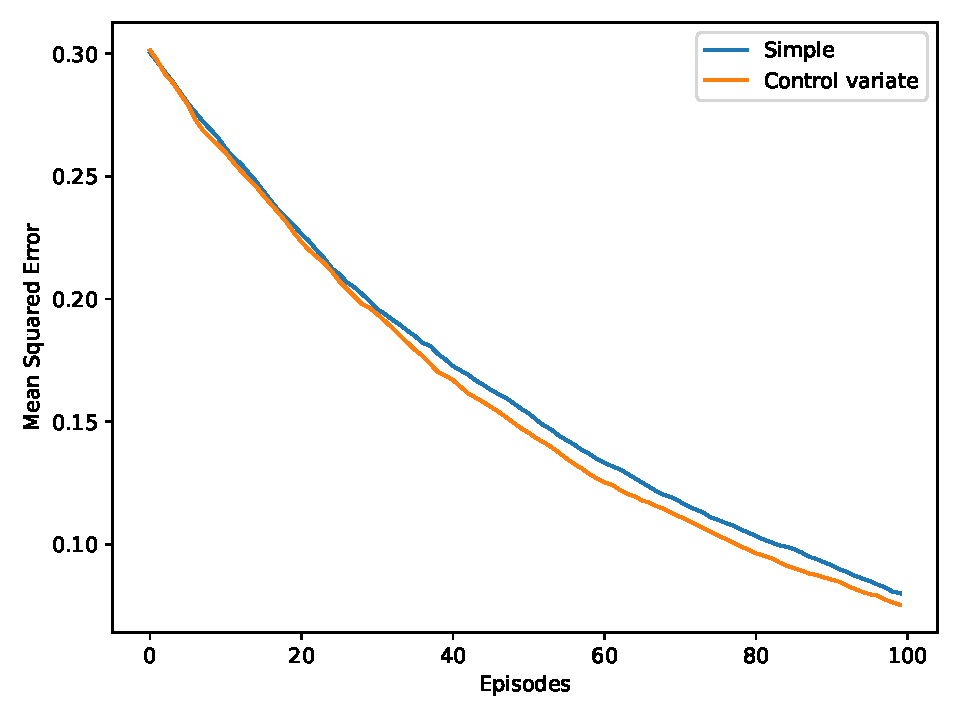
\includegraphics[width=0.8\textwidth]{chapters_latex/figures/ex_07_10.pdf}
    \captionsetup{labelformat=empty}
    \caption{Mean of the MSE after 100 episodes, averaged over 100 runs.}
\end{figure}